\lecture{Weak solutions: the three claims}{Lecture 2}{Math 6660 --- continues in the same OneNote export, from p.~7}

\begin{roadmap}[Lecture 2]
\roadq{Is the weak solution the same thing as the real solution?}
\begin{roadlist}
\item A weak solution is allowed to have a \textbf{kink}; a strong solution is
  not. The example: a bar whose $EA$ jumps at a point --- physically fine, but
  $u''$ does not exist there.
\item \textbf{Claim 1:} the weak solution is unique. One problem, one answer.
\item \textbf{Claim 2:} strong $\Rightarrow$ weak. Nothing is invented by going
  to the integral form.
\item \textbf{Claim 3:} weak $+$ enough smoothness $\Rightarrow$ strong. Nothing
  is lost either.
\end{roadlist}
\payoff{Trusting that the answer a virtual-work formulation produces is
\emph{the} answer, not an approximation to some neighbouring problem.}
\end{roadmap}

% ==================================================================
\subsection*{Setup, restated}

\paragraph{Two-point BVP.} On the fixed domain $0<x<1$:
\begin{equation}\label{eq:bvp2}
  -(au')' = f,
  \qquad u(0)=u(1)=0,
  \qquad \text{find } u\in\Ck[(0,1)]{2}.
\end{equation}

\paragraph{Variational formulation.}
\begin{equation}\label{eq:Vdef2}
  V = \left\{\, v \;:\;
    \int_{0}^{1} v^{2}\dx < \infty,\quad
    \int_{0}^{1} (v')^{2}\dx < \infty,\quad
    v(0)=v(1)=0 \,\right\}
  \qquad\text{(defining a space)}
\end{equation}

\noindent\textbf{Note.} Functions in $V$ are continuous
$\bigl(v\in\Ck[(0,1)]{0}\bigr)$.

\todoq{Page 7 of my notes writes the first condition as
$\int_{0}^{1}v^{2}\dx < 0$. That must be $<\infty$ --- the integrand is a
square, so $<0$ is impossible. Transcribed as $<\infty$.}

% ==================================================================
\subsection*{Example of a discontinuity}

Let
\begin{equation}\label{eq:H}
  H(x)=\begin{cases}
    1, & \tfrac14 < x < \tfrac34,\\[2pt]
    0, & \text{otherwise,}
  \end{cases}
\end{equation}
which is not continuous: $H\notin\Ck[(0,1)]{0}$, but $H\in \Ck[(0,1)]{-1}$ ---
it has a finite jump.

\begin{figure}[htbp]
\centering
\begin{tikzpicture}[scale=1.0, every node/.style={font=\small}]

% ================= (a) H(x) =================
\begin{scope}
  \draw[->,gray!70] (-0.3,0) -- (4.6,0) node[right,font=\scriptsize,black] {$x$};
  \draw[->,gray!70] (0,-0.3) -- (0,1.7);
  \draw[very thick,IntFrame] (0,0) -- (1,0);
  \draw[very thick,IntFrame] (1,1.1) -- (3,1.1);
  \draw[very thick,IntFrame] (3,0) -- (4,0);
  \draw[dotted,thick,PitFrame] (1,0) -- (1,1.1);
  \draw[dotted,thick,PitFrame] (3,0) -- (3,1.1);
  \draw[IntFrame,fill=white,thick] (1,0)   circle (1.9pt);
  \fill[IntFrame]                  (1,1.1) circle (1.9pt);
  \fill[IntFrame]                  (3,1.1) circle (1.9pt);
  \draw[IntFrame,fill=white,thick] (3,0)   circle (1.9pt);
  \draw[{Latex[length=1.5mm]}-{Latex[length=1.5mm]},PitFrame] (1.28,0.03) -- (1.28,1.07);
  \node[PitFrame,right,font=\scriptsize] at (1.33,0.55) {$+1$};
  \draw[{Latex[length=1.5mm]}-{Latex[length=1.5mm]},PitFrame] (2.72,1.07) -- (2.72,0.03);
  \node[PitFrame,left,font=\scriptsize] at (2.67,0.55) {$-1$};
  \foreach \x/\l in {0/0, 1/{\tfrac14}, 3/{\tfrac34}, 4/1}{
    \draw (\x,-0.09) -- (\x,0.09);
    \node[below,font=\scriptsize] at (\x,-0.11) {$\l$};}
  \node[left,font=\scriptsize] at (-0.07,1.1) {$1$};
  \node[font=\small] at (2.0,2.05) {\textbf{(a)} $H(x)$ --- the displacement};
\end{scope}

% ================= (b) the bar =================
\begin{scope}[shift={(6.4,0)}]
  \fill[IntBack] (0,0) rectangle (0.9,0.42);   \draw[thick] (0,0) rectangle (0.9,0.42);
  \fill[MEBack]  (1.1,0) rectangle (2.9,0.42); \draw[thick] (1.1,0) rectangle (2.9,0.42);
  \fill[IntBack] (3.1,0) rectangle (4,0.42);   \draw[thick] (3.1,0) rectangle (4,0.42);
  \draw[decorate,decoration={zigzag,segment length=3pt,amplitude=1.6pt},PitFrame,thick]
        (1.0,-0.12) -- (1.0,0.54);
  \draw[decorate,decoration={zigzag,segment length=3pt,amplitude=1.6pt},PitFrame,thick]
        (3.0,-0.12) -- (3.0,0.54);
  \node[PitFrame,font=\scriptsize,align=center] at (1.0,-0.5) {break};
  \node[PitFrame,font=\scriptsize,align=center] at (3.0,-0.5) {break};
  \node[font=\scriptsize] at (0.45,0.21) {$u=0$};
  \node[font=\scriptsize] at (2.0,0.21)  {$u=1$};
  \node[font=\scriptsize] at (3.55,0.21) {$u=0$};
  \node[font=\small] at (2.0,2.05) {\textbf{(b)} two clean breaks};
  \node[font=\scriptsize,align=center,MEFrame] at (2.0,1.25)
       {the middle half has moved bodily;\\ the bar is in three pieces};
\end{scope}

% ================= (c) H'(x) : deltas =================
\begin{scope}[shift={(0,-3.9)}]
  \draw[->,gray!70] (-0.3,0) -- (4.6,0) node[right,font=\scriptsize,black] {$x$};
  \draw[->,gray!70] (0,-1.35) -- (0,1.35);
  \draw[very thick,IntFrame] (0,0) -- (0.95,0);
  \draw[very thick,IntFrame] (1.05,0) -- (2.95,0);
  \draw[very thick,IntFrame] (3.05,0) -- (4,0);
  \draw[very thick,-{Latex[length=2.6mm]},PitFrame] (1,0) -- (1,1.05);
  \draw[very thick,-{Latex[length=2.6mm]},PitFrame] (3,0) -- (3,-1.05);
  \node[PitFrame,right,font=\scriptsize] at (1.08,0.85)  {$+\delta_{1/4}$};
  \node[PitFrame,right,font=\scriptsize] at (3.08,-0.85) {$-\delta_{3/4}$};
  \foreach \x/\l in {1/{\tfrac14}, 3/{\tfrac34}}{
    \draw (\x,-0.08) -- (\x,0.08);}
  \node[font=\small] at (2.0,1.75) {\textbf{(c)} $H'=\delta_{1/4}-\delta_{3/4}$};
  \node[font=\scriptsize,PitFrame] at (2.0,-1.65) {height $\infty$, area $\pm1$};
\end{scope}

% ================= (d) smoothed H_h' =================
\begin{scope}[shift={(6.4,-3.9)}]
  \draw[->,gray!70] (-0.3,0) -- (4.6,0) node[right,font=\scriptsize,black] {$x$};
  \draw[->,gray!70] (0,-1.35) -- (0,1.35);
  \fill[IntBack] (0.78,0) rectangle (1.22,1.05);
  \fill[MEBack]  (2.78,0) rectangle (3.22,-1.05);
  \draw[very thick,IntFrame] (0,0) -- (0.78,0) -- (0.78,1.05) -- (1.22,1.05) -- (1.22,0)
        -- (2.78,0) -- (2.78,-1.05) -- (3.22,-1.05) -- (3.22,0) -- (4,0);
  \node[right,font=\scriptsize] at (1.26,1.05)  {$+1/h$};
  \node[right,font=\scriptsize] at (3.26,-1.05) {$-1/h$};
  \draw[decorate,decoration={brace,amplitude=3pt,mirror},thin] (0.78,-0.16) -- (1.22,-0.16);
  \node[below,font=\scriptsize] at (1.0,-0.32) {$W_{1}$};
  \draw[decorate,decoration={brace,amplitude=3pt},thin] (2.78,0.16) -- (3.22,0.16);
  \node[above,font=\scriptsize] at (3.0,0.3) {$W_{2}$};
  \node[font=\small] at (2.0,1.75) {\textbf{(d)} smoothed $H_{h}'$, width $h$};
  \node[font=\scriptsize,MEFrame,align=center] at (2.0,-1.7)
       {$W_{1}\cap W_{2}=\varnothing$ for $h<\tfrac12$\\ $\Rightarrow$ cross term $=0$};
\end{scope}

\end{tikzpicture}
\caption{The step $H$: (a) the displacement field, jumping $+1$ then $-1$;
(b) the same thing as a bar --- three pieces, two breaks; (c) its derivative,
a pair of deltas; (d) the smoothed version used for the honest calculation.}
\label{fig:step}
\end{figure}

So
\begin{equation}
  \int_{0}^{1} H^{2}\dx = \int_{1/4}^{3/4}\dx = \tfrac12 \;<\;\infty .
\end{equation}
The first condition in \eqref{eq:Vdef2} is satisfied. Now the derivative:
\begin{equation}\label{eq:Hprime}
  H'(x) = \delta\!\left(x-\tfrac14\right) - \delta\!\left(x-\tfrac34\right)
        \;=\; \delta_{1/4} - \delta_{3/4},
\end{equation}
writing $\delta_{1/4}\equiv\delta(x-\tfrac14)$ and
$\delta_{3/4}\equiv\delta(x-\tfrac34)$ --- the same objects, shorter names.
Each jump contributes one delta, sited at the jump, with coefficient equal to
the \emph{signed} jump size:
\begin{center}\small
\renewcommand{\arraystretch}{1.2}
\begin{tabular}{@{}llll@{}}
\toprule
\textbf{at} & \textbf{$H$ goes} & \textbf{size} & \textbf{contributes}\\
\midrule
$x=\tfrac14$ & $0\to1$ & $+1$ & $+\,\delta_{1/4}$\\
$x=\tfrac34$ & $1\to0$ & $-1$ & $-\,\delta_{3/4}$\\
\bottomrule
\end{tabular}
\end{center}

\begin{recall}[$\delta$ properties]
For $\delta(x-x_{0})$:
\begin{align}
  \int_{x_{0}-\eps_{1}}^{x_{0}+\eps_{2}} \delta(x-x_{0})\dx &= 1
    \qquad\text{for any }\eps_{1},\eps_{2}>0, \label{eq:delta1}\\[4pt]
  \int_{x_{0}-\eps_{1}}^{x_{0}+\eps_{2}} f(x)\,\delta(x-x_{0})\dx &= f(x_{0}),
    \qquad f \text{ a continuous function.} \label{eq:delta2}
\end{align}
\end{recall}

Now expand the square --- three terms, and \emph{all three} must be accounted
for:
\begin{align}\label{eq:Hsq}
  \int_{0}^{1}(H')^{2}\dx
    &= \int_{0}^{1}\left(\delta_{1/4}-\delta_{3/4}\right)^{2}\dx \notag\\[2pt]
    &= \int_{0}^{1}\underbrace{\delta_{1/4}^{2}}_{\text{(i)}}\dx
       \;-\;2\!\int_{0}^{1}\underbrace{\delta_{1/4}\,\delta_{3/4}}_{\text{(ii)}}\dx
       \;+\;\int_{0}^{1}\underbrace{\delta_{3/4}^{2}}_{\text{(iii)}}\dx .
\end{align}
An arrow is then drawn from term (i) down to the assertion
\begin{equation}\label{eq:sq1}
  \int_{0}^{1}\delta\!\left(x-\tfrac14\right)\delta\!\left(x-\tfrac14\right)\dx
  = +\infty ,
\end{equation}
and the conclusion $H\notin V$ follows immediately.

\todoq{Two gaps here, both in the lecture as written. \textbf{(a)} No
justification is offered for \eqref{eq:sq1} --- and \eqref{eq:delta2} cannot
supply one, since it requires $f$ to be a \emph{continuous function} while
$\delta$ is not a function at all, so $f=\delta$ is not a legal substitution.
\textbf{(b)} Only term (i) is touched; (ii) and (iii) are never addressed. The
\emph{conclusion} \eqref{eq:sq1} is correct --- the derivation below supplies
what is missing.}

% ------------------------------------------------------------------
\paragraph{The honest computation.}
Replace each jump by a ramp of width $h$. Then $H_{h}'$ is an ordinary
piecewise-constant \emph{function}:
\begin{equation}\label{eq:Hh}
  H_{h}'(x)=\begin{cases}
    +1/h, & x\in W_{1}=\left(\tfrac14-\tfrac h2,\ \tfrac14+\tfrac h2\right),\\[3pt]
    -1/h, & x\in W_{2}=\left(\tfrac34-\tfrac h2,\ \tfrac34+\tfrac h2\right),\\[3pt]
    0,    & \text{elsewhere,}
  \end{cases}
  \qquad\text{and for } h<\tfrac12,\ \ W_{1}\cap W_{2}=\varnothing .
\end{equation}
Now every term of \eqref{eq:Hsq} can be evaluated with no distributions at all:
\begin{center}\small
\renewcommand{\arraystretch}{1.35}
\begin{tabular}{@{}clll@{}}
\toprule
 & \textbf{term} & \textbf{smoothed integrand} & \textbf{integral}\\
\midrule
(i)   & $\delta_{1/4}^{2}$              & $(1/h)^{2}$ on $W_{1}$, else $0$
      & $\dfrac{1}{h^{2}}\cdot h=\dfrac1h$\\
(ii)  & $-2\,\delta_{1/4}\delta_{3/4}$  & $0$ everywhere ($W_{1}\cap W_{2}=\varnothing$)
      & $0$\\
(iii) & $\delta_{3/4}^{2}$              & $(-1/h)^{2}$ on $W_{2}$, else $0$
      & $\dfrac{1}{h^{2}}\cdot h=\dfrac1h$\\
\midrule
      & \textbf{total} & &
        $\dfrac1h+0+\dfrac1h=\dfrac{2}{h}\ \longrightarrow\ \infty$\\
\bottomrule
\end{tabular}
\end{center}

\noindent
Note (ii): the cross term vanishes for a \emph{rigorous} reason, not a
hand-wave --- the two windows are disjoint, so wherever one factor is nonzero
the other is zero. \textbf{Deltas at different places never interact.} And
(iii) contributes $+1/h$, not $-1/h$: the sign is destroyed by the square, so
the two spikes \emph{add}.

\begin{intuition}[finite area, infinite squared area]
No sampling property is needed anywhere. The one fact is
\[
  \int \delta\dx = 1 \quad\text{(finite \textbf{area})},
  \qquad\text{but}\qquad
  \int \delta^{2}\dx = \infty .
\]
A delta has finite area but \textbf{infinite height}; squaring the height beats
the shrinking width. Seen in the smoothed numbers, with $H=1/h$ and $W=h$:
\[
  \underbrace{H\cdot W = \tfrac1h\cdot h = 1}_{\text{plain: the }h\text{'s cancel}}
  \qquad\text{vs.}\qquad
  \underbrace{H^{2}\cdot W = \tfrac{1}{h^{2}}\cdot h = \tfrac1h}_{\text{squared: one }h\text{ survives below}}
\]
\end{intuition}

\begin{recall}[the plain integral passes --- as always]
Run \eqref{eq:Hh} through the \emph{unsquared} test as a control:
\[
  \int_{0}^{1}H_{h}'\dx
  = \underbrace{\left(+\tfrac1h\right)h}_{W_{1}}
  + \underbrace{\left(-\tfrac1h\right)h}_{W_{2}}
  = 1-1 = 0
  \;=\; H(1)-H(0)\quad\text{\cmark\ (FTC)} .
\]
Finite for every $h$, and independent of $h$. So the plain condition would
\emph{admit} this broken bar. Only the square rejects it.
\end{recall}

\noindent Therefore
\begin{equation}
  \boxed{\;H(x)\notin V\;}
  \qquad\text{because } H' \text{ is not square integrable.}
\end{equation}

\begin{mechanics}[the calculation behind ``the bar is broken'']
$H$ is a bar whose middle half has been translated bodily by $1$ --- two clean
breaks, at $x=\tfrac14$ and $x=\tfrac34$. Its ``strain'' $H'$ is a pair of
deltas: infinite strain at the two break points, so
$\int(H')^{2}=+\infty$ and $H$ is excluded from $V$.

Note \emph{which} test it passes and which it fails:
\begin{center}\small
\begin{tabular}{@{}lll@{}}
\toprule
test & value & verdict\\
\midrule
$\int H^{2}\dx$      & $\tfrac12$ & finite \cmark\ --- the displacement is perfectly reasonable\\
$\int H'\dx$         & $0$        & finite \cmark\ --- the plain derivative test too\\
$\int (H')^{2}\dx$   & $\infty$   & \xmark\ --- \textbf{only the energy condition rejects it}\\
\bottomrule
\end{tabular}
\end{center}
That is the precise sense in which ``finite strain energy'' is a stronger and
more physical requirement than ``bounded''.
\end{mechanics}

\begin{pitfall}[use the smoothing version in a proof]
$\delta^{2}$ is genuinely undefined --- the product of two distributions has no
meaning in general, so \eqref{eq:sq1} cannot be justified as it stands. If a
step like it appears in your own work, write the smoothed version
\eqref{eq:Hh} and take $h\to0$: same conclusion, every object an ordinary
function.
\end{pitfall}

% ==================================================================
\subsection*{The variational problem}

\begin{equation}\label{eq:varprob}
  \text{Find } u\in V \text{ such that }
  \int_{0}^{1} a\,u'v'\dx = \int_{0}^{1} f v\dx
  \qquad \text{for all } v\in V.
\end{equation}

\noindent\textbf{Note.} $u$ is the \emph{trial} function; $v$ are the
\emph{test} functions. In this case $u$ and $v$ come from the same function
space, $V$.

\begin{intuition}[this is the principle of virtual work]
Read it term by term with $a=EA$, $u'=\eps$, $v=\delta u$, $v'=\delta\eps$:
\[
  \underbrace{\int_{0}^{1} \underbrace{a u'}_{\sigma A}\;
    \underbrace{v'}_{\delta\eps}\dx}_{\text{internal virtual work}}
  \;=\;
  \underbrace{\int_{0}^{1} f\,\underbrace{v}_{\delta u}\dx}_{\text{external virtual work}}
\]
The test function is the virtual displacement. ``For all $v\in V$'' is
``for every kinematically admissible virtual displacement.'' The whole statement
is $\delta W_{\text{int}} = \delta W_{\text{ext}}$ --- equilibrium.

You have used this since undergraduate statics. What the math department adds
is not the equation but the precision about \emph{which space} $u$ and $v$ live
in, and that turns out to be the thing that makes the theory work.
\end{intuition}

\begin{pitfall}[trial $=$ test only because the BCs are homogeneous]
The note ``$u$ and $v$ come from the same function space'' is true \emph{here}
and not in general. It holds because $u(0)=u(1)=0$: the prescribed displacement
happens to be zero.

With a nonhomogeneous essential BC, say $u(0)=g\ne0$, the trial function must
satisfy $u(0)=g$ while the test function must satisfy $v(0)=0$ --- the virtual
displacement cannot violate the support. So the trial set is an affine shift of
the test space, not the same space, and it is not even a vector space. The
standard fix is to write $u = \tilde u + u_{g}$ with $\tilde u\in V$, which is
exactly what a solver does internally when it eliminates prescribed DOFs and
moves their contribution to the right-hand side.
\end{pitfall}

\medskip
\noindent\textbf{Q: How are (2-pt BVP) and (variational problem) related?}
\begin{itemize}[leftmargin=1.6em,itemsep=1pt]
  \item BVP requires $u\in\Ck[(0,1)]{2}$.
  \item Variational problem only needs $u\in V$.
\end{itemize}

\begin{intuition}[the question the next three claims answer]
Two different problems are now on the table, and they demand different amounts
of smoothness. The natural worry is whether we have quietly changed the
problem. Claims 1--3 settle it:
\begin{itemize}[leftmargin=1.4em,itemsep=2pt]
  \item \textbf{Claim 1}: the variational problem has at most one solution.
  \item \textbf{Claim 2}: every BVP solution solves the variational problem
        (the weak form is not \emph{more} restrictive).
  \item \textbf{Claim 3}: under extra smoothness, every variational solution
        solves the BVP (a partial converse).
\end{itemize}
Claim 3 needs hypotheses that Claim 2 does not. That gap is not a defect of the
proof --- it is where \emph{weak solutions} live, and the final note of the
lecture names it.
\end{intuition}

% ==================================================================
\subsection*{Claim 1: uniqueness}

\begin{proposition}
If the variational problem has a solution, it is unique.
\end{proposition}

\begin{proof}[Proof (by contradiction)]
Assume there exist 2 different solutions, $u$ and $U$:
\[
  \int_{0}^{1} a u'v'\dx = \int_{0}^{1} fv\dx
  \qquad\Big|\qquad
  \int_{0}^{1} a U'v'\dx = \int_{0}^{1} fv\dx .
\]
Then subtract:
\begin{equation}
  \Rightarrow\quad \int_{0}^{1} a\,(u-U)'\,v'\dx = 0 .
\end{equation}
Take $v = u-U \in V$. Now
\begin{equation}\label{eq:zeroenergy}
  \int_{0}^{1} a\Bigl((u-U)'\Bigr)^{2}\dx = 0
  \quad\Longrightarrow\quad (u-U)' = 0 \ \text{ on } (0,1)
  \quad\Longrightarrow\quad u = U + c .
\end{equation}
But by the BCs, $c=0$, so $u=U$.
\end{proof}

\begin{intuition}[a zero-energy difference is a rigid body motion]
Follow \eqref{eq:zeroenergy} mechanically. Suppose two different displacement
fields both equilibrate the same load. Their difference $u-U$ is then a shape
that stores \emph{zero} strain energy --- the integrand is
$a\cdot(\text{strain})^{2}$ with $a\ge a_{1}>0$, so the only way the integral
vanishes is if the strain vanishes everywhere.

Zero strain everywhere means the difference is a rigid body motion: $u-U=c$, a
uniform translation. And the supports forbid that, so $c=0$.

This is the continuum version of ``$\Kmat$ positive definite $\Rightarrow$
$\Kmat\bm{U}=\bm{F}$ has a unique solution,'' and note precisely where each
hypothesis is spent: $a\ge a_{1}>0$ gives \emph{positive} definiteness (energy
is zero only for zero strain), and the boundary conditions remove the
rigid-body null space. Drop either one and uniqueness fails --- which is exactly
what a solver tells you when it reports a singular stiffness matrix.
\end{intuition}

\begin{remark}
The lecturer labels this ``by contradiction,'' but no contradiction is actually
reached --- the argument derives $u=U$ directly. It is a direct uniqueness
proof.
\end{remark}

% ==================================================================
\subsection*{Claim 2: BVP $\Rightarrow$ variational}

\begin{proposition}
A solution to the BVP is a solution to the variational problem.
\end{proposition}

\begin{proof}
The BVP has a unique solution $u\in\Ck[(0,1)]{2}$ with $u(0)=u(1)=0$.
If $u\in\Ck[(0,1)]{2}$ and satisfies the BCs, then $u\in V$. The BVP and the
variational problem are then equivalent via integration by parts.
\end{proof}

\begin{intuition}[the easy direction, and why it is easy]
$C^{2}$ functions on a bounded interval have bounded derivatives, so
$\int (u')^{2}$ is certainly finite --- a classical solution automatically has
finite strain energy. Add the BCs and it lands in $V$. Then
\eqref{eq:mult}--\eqref{eq:ibp1d} run forward with no extra hypotheses.

The direction that costs something is the other one: going from ``the integral
identity holds for every $v$'' back to ``the differential equation holds
pointwise.'' That is Claim 3, and it needs both extra regularity \emph{and} a
genuine argument.
\end{intuition}

% ==================================================================
\subsection*{Claim 3: variational $\Rightarrow$ BVP}

\begin{proposition}\label{prop:claim3}
If $f\in\Ck[(0,1)]{0}$, $a\in\Ck[(0,1)]{1}$, and
$0<a_{1}\le a(x)\le a_{2}<\infty$ for all $x\in(0,1)$, then a solution to the
variational problem is a solution to the BVP.
\end{proposition}

\begin{proof}
Assume for the moment that $u\in\Ck[(0,1)]{2}$. From \eqref{eq:varprob},
\begin{equation}
  \int_{0}^{1}\bigl(a u'v' - fv\bigr)\dx = 0 .
\end{equation}
Reverse integration by parts:
\begin{equation}\label{eq:Sdef}
  \int_{0}^{1}\underbrace{\Bigl[(au')' + f\Bigr]}_{S(x)} v\dx = 0 .
\end{equation}

\noindent\textbf{Goal:} show $S(x)=0$ for all $x\in(0,1)$.

\medskip
\noindent\textbf{(a)} Assume, for contradiction, that
\[
  S(\xi) = \Bigl[(au')'+f\Bigr]\Big|_{x=\xi} > 0
  \qquad\text{at some point } \xi\in(0,1).
\]
Note that $S(x)$ is continuous in $x$. By continuity, $S(x)>0$ for
$x\in[\xi-\delta,\,\xi+\delta]$ for some $\delta>0$.

Choose $v$ to be the following ``hat'' function:
\begin{center}
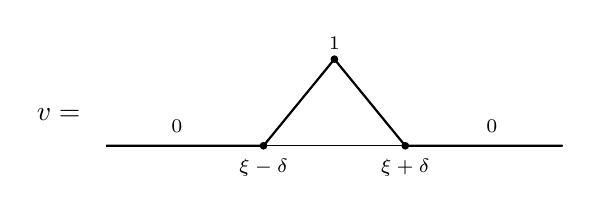
\begin{tikzpicture}[scale=1.0]
  \draw[-] (-0.4,0) -- (5.4,0);
  \draw[thick] (-0.4,0) -- (1.6,0) -- (2.5,1.1) -- (3.4,0) -- (5.4,0);
  \fill (1.6,0) circle (1.4pt);
  \fill (3.4,0) circle (1.4pt);
  \fill (2.5,1.1) circle (1.4pt);
  \node[above] at (2.5,1.1) {\scriptsize$1$};
  \node[below] at (1.6,-0.05) {\scriptsize$\xi-\delta$};
  \node[below] at (3.4,-0.05) {\scriptsize$\xi+\delta$};
  \node[above] at (0.5,0.05) {\scriptsize$0$};
  \node[above] at (4.5,0.05) {\scriptsize$0$};
  \node[left] at (-0.6,0.4) {$v=$};
\end{tikzpicture}
\end{center}
But then
\[
  \int_{0}^{1} S(x)\,v(x)\dx > 0,
\]
which is a contradiction with \eqref{eq:Sdef}. Therefore $S(x)$ cannot be
positive in $(0,1)$.

\medskip
\noindent\textbf{(b)} Redo this argument with $S(\xi)<0$
$\Rightarrow$ $S(x)$ cannot be negative in $(0,1)$.

\medskip
Hence $S\equiv0$, which is \eqref{eq:bvp2}.
\end{proof}

\begin{intuition}[the hat function is not a coincidence]
Two things are worth pausing on here.

\textbf{First, the logic.} This is the \emph{fundamental lemma of the calculus
of variations}: if $\int S v = 0$ for \emph{every} admissible $v$, then $S=0$.
The mechanical reading is the converse of virtual work --- if a leftover force
distribution $S$ does zero virtual work against every admissible virtual
displacement, there is no leftover force. The proof makes that concrete by
picking a virtual displacement that pokes the bar \emph{only} where $S$ is
claimed to be positive, so the work integral cannot cancel.

\textbf{Second, the choice of $v$.} The bump used to localise is the hat
function --- a piecewise-linear tent, one at $\xi$, zero outside
$[\xi-\delta,\xi+\delta]$. That is precisely the linear finite element basis
function $\phih_{i}$ you will build $\Vh$ from in a few lectures, and precisely
why the stiffness matrix comes out sparse (each hat overlaps only its
neighbours).

So the object introduced here as a proof device is the same object that becomes
the computational method. Worth noticing now: it is also the cleanest evidence
that $V$ was built to contain kinked functions, since a hat has no second
derivative at its peak and belongs to $V$ anyway.
\end{intuition}

\begin{pitfall}[the proof assumes what it is trying to conclude]
The proof opens with ``assume for the moment that $u\in C^{2}(0,1)$'' --- but
$u\in C^{2}$ is essentially the conclusion of Proposition~\ref{prop:claim3}.
As written, the argument shows: \emph{if} a variational solution happens to be
$C^{2}$, \emph{then} it satisfies the BVP pointwise.

Closing that gap --- proving the regularity rather than assuming it --- is a
separate theorem (elliptic regularity), and the hypotheses $f\in C^{0}$,
$a\in C^{1}$ are exactly what it needs. The lecturer's ``for the moment''
signals the debt. The final note below is where it gets paid.
\end{pitfall}

% ==================================================================
\subsection*{When can we expect $u\in\Ck[(0,1)]{2}$?}

\begin{equation}\label{eq:star}
  (\star)\qquad
  f\in\Ck[(0,1)]{0},\quad
  a\in\Ck[(0,1)]{1},\quad\text{and}\quad
  0<a_{1}\le a(x)\le a_{2}<\infty
  \quad \forall\, x\in(0,1).
\end{equation}

\noindent\textbf{Note.}
\begin{enumerate}[label=\textcircled{\scriptsize\arabic*},leftmargin=2.2em,itemsep=6pt]
  \item If $(\star)$ is satisfied: $u$ is a \emph{strong} solution of the
        2-pt BVP, and
        \[
          (\text{2-pt BVP}) \;\equiv\; (\text{variational problem}).
        \]
  \item If $(\star)$ is \emph{not} satisfied, the 2-pt BVP will not have a
        solution, but the variational problem may still have one.
        Then $u$ (if it exists) is a \emph{weak} solution of the 2-pt BVP.
\end{enumerate}

\begin{intuition}[case \textcircled{\scriptsize2} is the whole reason for the course]
This is the payoff, and it is worth stating in engineering terms because it
describes a situation you have already simulated.

Take a bar made of two materials --- steel for $x<\tfrac12$, aluminium for
$x>\tfrac12$. Then $a(x)$ \emph{jumps} at the interface, so $a\notin C^{1}$
and $(\star)$ fails. Consequently:
\begin{itemize}[leftmargin=1.4em,itemsep=2pt]
  \item The strong form has \textbf{no solution}. Not ``a hard one'' --- none.
        $u''$ does not exist at the interface, so $-(au')'=f$ is meaningless
        there.
  \item The variational problem is \textbf{completely fine}. It never asked for
        $u''$. It asks for finite strain energy, and a bimaterial bar plainly
        has that.
\end{itemize}
The physically correct answer --- displacement continuous, internal force
$au'$ continuous, strain $u'$ jumping at the interface --- is a weak solution
and not a strong one.

So the weak formulation is not a relaxation adopted for convenience. It is the
formulation under which the problem you actually want to solve \emph{has} an
answer. Every real FE model with more than one material, a contact interface, or
a point load lives in case \textcircled{\scriptsize2}.
\end{intuition}

\begin{pitfall}[``will not have a solution'' is slightly too strong]
$(\star)$ is a \emph{sufficient} condition for $u\in C^{2}$, not a necessary
one, so its failure does not by itself prove that no classical solution exists
--- one might survive by luck. The accurate statement is that the BVP
\emph{need not} have a classical solution when $(\star)$ fails, while the
variational problem still can. The bimaterial bar is a case where it genuinely
does fail.
\end{pitfall}

\begin{dictionary}[strong vs.\ weak]
strong solution & the classical one: $u\in C^{2}$, the PDE holds at every point \\
weak solution & the physical one: finite strain energy, equilibrium holds in the virtual-work sense \\
$(\star)$ fails & material interface, point load, re-entrant corner, contact \\
$u$ solves the variational problem & the structure is in equilibrium against every admissible virtual displacement \\
\end{dictionary}

\begin{intuition}[what the course has actually set up]
Standing back from Lectures 1--2, a chain has been built and it is worth
naming, because everything later hangs off it:
\[
  \underbrace{-(au')'=f}_{\text{strong form}}
  \;\longrightarrow\;
  \underbrace{\int a u'v' = \int fv \ \ \forall v\in V}_{\text{weak form}}
  \;\longrightarrow\;
  \underbrace{\text{same, with } V \text{ replaced by } \Vh}_{\text{Galerkin / FEM}}
\]
The first arrow is what these two lectures did: it costs nothing (Claims 2 and
3) and buys a problem that is solvable in realistic situations. The second arrow
has not happened yet --- it is where approximation enters, and where
$\int a u'v'$ becomes the stiffness matrix $K_{ij} = \int a\phih_{j}'\phih_{i}'$.

Keep the two arrows separate. ``Weak'' refers to the first and involves no
approximation whatsoever; the error you eventually measure comes entirely from
the second.
\end{intuition}
